\chapter{Hawkes Process}
In this chapter, we introduce a class of processes in which the event arrival rate explicitly depends on past events – i.e. self-exciting processes – and we further detail the most well-known self-exciting process, the Hawkes process.
\section{Hawkes process definition}
\begin{Definition}[{\cite[pp.9]{Hawkess}}(Hawkes process definition)]{}	
	Considers $(N(t): t\in R)$ a counting process, with associated history $(H(t):
	t \in R)$, that satisfies
	\begin{align*}
	P(N(t + h) - N(t) = m \rvert N(t)) = 
	\begin{cases*}
	\lambda^{*}(t)h & $m = 1$ \\
	o(h) & $m > 1$  \\
	1-\lambda^{*}(t)h + o(h) & $ m = 0$  
	\end{cases*}  
	\end{align*}
Suppose the process’conditional intensity function is of the form
	\begin{align*}
	\lambda^{*}(t) = \lambda + \displaystyle\int\limits_{-\infty}^{t} \mu(t-u)dN(u) 
	\end{align*}
for some $\lambda \in R^{+}$ and $\mu: R^{+} \rightarrow R^{+} \cup {0}$ which are called the background intensity and excitation function respectively. Such a process $N(.)$ is a Hawkes process.
\end{Definition}

There are two major simulation approaches in the literature such as intensity-based and cluster-based, since a Hawkes process can be defined via a conditional stochastic intensity function.

\section{Intensity-based Hawkes Process Model}

\subsection{Hawkes conditional intensity function}
\begin{Definition}[{\cite[pp.10-11]{Hawkess}}(conditional intensity function)]{}	
	The observed sequence of past arrival times of the point process up to time $t$, the Hawkes conditional intensity is
	$$\lambda^{*}(t) = \lambda + \sum_{t_{i} < t} \mu (t-t_{i})$$
	In this case $\mu(.)$ is specified by constants $\alpha, \beta \in R^{+}$ such that
	\begin{align}
	\label{Def_HakessIntensity}
	\lambda^{*}(t) = &
	\lambda + \displaystyle\int\limits_{-\infty}^{t} \alpha e^{-\beta(t-s)}dN(s) 
	\\
	& = \lambda + \sum_{t_{i} < t}\alpha e^{-\beta(t-t_{i})} \nonumber
	\end{align}
	with each arrival in the system instantaneously increases the arrival intensity by $\alpha$, then over time this arrival’s influence decays at rate $\beta$.
\end{Definition}
If the Hawkes process is restricted to $R^{+}$ with
some initial condition $\lambda^{*}(0) = \lambda_{0}$ then the conditional intensity process satisfies the
stochastic differential equation
$$d\lambda^{*}(t) = \beta(\lambda - \lambda^{*}(t))dt + \alpha dN(t) , t \geq 0 .$$
	Applying stochastic calculus to yield the general solution of	
		\begin{align*}
		\lambda^{*}(t) = e^{-\beta t} (\lambda_{0} - \lambda) +\lambda + \displaystyle\int_{0}^{t} \alpha e^{\beta(t-s)}dN(s), t \geq 0. 
		\end{align*}
	which is a natural extension of Eq. \ref{Def_HakessIntensity}.
	


\subsection{Algorithm}
Ogata (1981) proposes an algorithm for the simulation of Hawkes processes. The conditional intensity $\lambda^{*}(.)$ does not have an asymptotic upper bound, however it is common for the intensity to be non-increasing in periods without any arrivals. This implies that for $t \in (T_{i}, T_{i+1}], \lambda^{*}(t) \leq \lambda^{*}(T_{i}^{+})$. So the $M$ value can be updated during each simulation. This algorithm describes Hawkes process by thinning.
\begin{breakablealgorithm}
	\caption{Generate an Hawkes process by thinning}
	\label{Alg:Hawkes_Thinning}
	\begin{algorithmic}[H] \item
		\begin{tabbing}
			INPUT:  \=
			\\
			\> $T$: the sequence of random arrival times.
			\\
			\>$\lambda(.)$: the intensity function.
			\\
			OUTPUT: 
			\\
			\> $P$: retrieve the simulated process on $ [0, T ]$.
			\\
			1.\= \textbf{Procedure} HawkesByThinning $(T,\lambda(.))$
			\\
			2.\textbf{Require}: $\lambda^{*}(t)$ non-increasing in periods of no arrivals.
			\\
			\hspace{0.5cm} $ \varepsilon \leftarrow 10^{-10}$ (some tiny value $> 0$ )
			\\
			\hspace{0.5cm} $P \leftarrow [], t \leftarrow 0.$
			\\
			3.\textbf{General routine}
			\\
			\hspace{0.5cm}\textbf{while} $t < T $ \textbf{do}
			\\
			\hspace{1cm}Find new upper bound: $M \leftarrow \lambda^{*}(t + \varepsilon)$.
			\\
			\hspace{1cm}Generate next candidate point: $E \leftarrow Exp(M)$, $ t \leftarrow t + E $
			\\
			\hspace{1cm}Keep it with some probability: $U \leftarrow Unif(0,M)$.
			\\
			\hspace{1cm}\textbf{if} $t < T$ \textbf{and} $U \leq \lambda^{*}(t) $ \textbf{then}
			\\
			\hspace{1.5cm}$P \leftarrow [P, t].$
			\\
			\hspace{1cm}\textbf{end if}
			\\
            \hspace{0.5cm}\textbf{end while}
			\\
			\hspace{0.5cm}\textbf{return} $P$
			\\
			\hspace{0.2cm}\= \textbf{End procedure}
		\end{tabbing}
	\end{algorithmic}
\end{breakablealgorithm}
\subsection{Example}

Let us simulate Hawkes process, using Algorithm \ref{Alg:Hawkes_Thinning}. For set values of $T=30, \lambda = 0.5, \alpha=0.15, \beta=1$, we obtained a Hawkes (self-exciting) process; a graph of its intensity, along with
the event times, is presented in Figure \ref{Example_Thinning}. We see that as defined an arrival (an event) causes the conditional intensity function to increase.

  \begin{figure}[H]
  	\centering
  	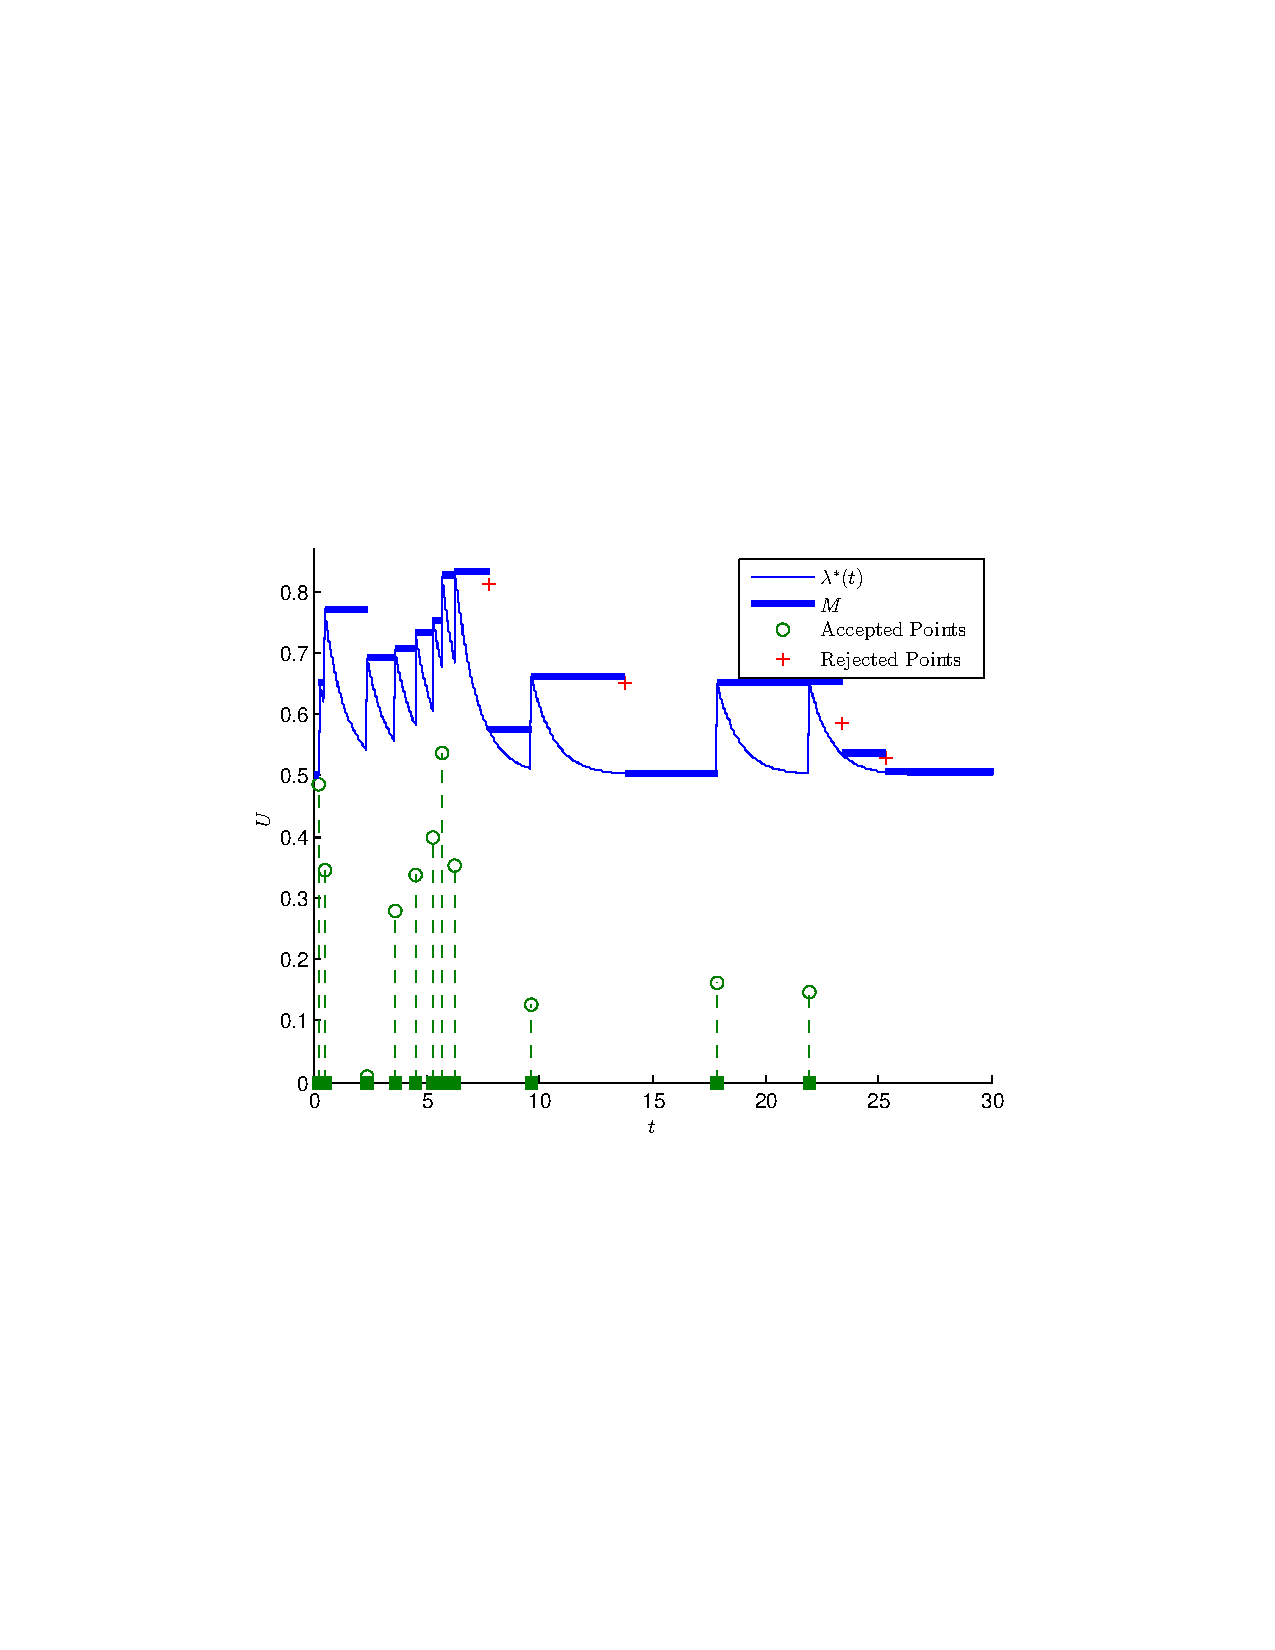
\includegraphics[trim = 0.8cm 8.5cm 0.8cm 8cm,clip,width=1.00\textwidth ]{Hawkess_Thinning.pdf}
  	\caption{A simulation of process by thinning.}
  	\label{Example_Thinning}
  \end{figure}
Figure \ref{Example_Thinning} presents A Hawkes process with $(\lambda, \alpha, \beta) =
(0.5, 0.15, 1)$. Each $(t, U)$ point describes a suggested arrival at time $t$ whose $U$ value
is given in Algorithm \ref{Alg:Hawkes_Thinning}. Plus signs signs indicate rejected points, circles accepted, and green squares the resulting point processes.

\section{Cluster-based Hawkes Process Model}

\subsection{Immigration–birth representation}
 Imagine counting the population in a country where people
 arrive either via immigration or by birth. Say that the stream of immigrants to the country form a homogeneous Poisson process at rate $\lambda$. Each person then produces zero or more children in an independent and identify distribution, the arrival of births form an non-homogeneous Poisson process.
  \begin{figure}[H]
  	\centering
  	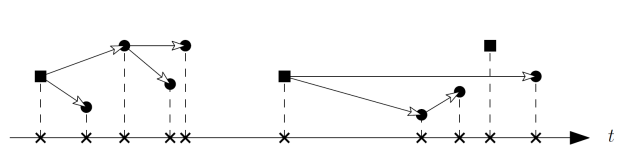
\includegraphics[width=0.8\textwidth]{Immigrate_Birth.PNG}
  	\caption{Hawkes process represented as a collection of family trees (immigration–
  		birth representation).}
 
  	\label{Immigrate_Birth}
  \end{figure}
  Squares indicate immigrants, circles are offspring/descendants, and the crosses denote the generated point process
\subsection{Algorithm}
The immigration–birth representation gives rise to a simple simulation procedure: generate the immigrant arrivals, then generate the descendants for each immigrant. This algorithm describes Hawkes process by cluster.
\begin{breakablealgorithm}
	\caption{Generate an Hawkes process by clusters}
	\label{Alg:Hawkes_clusters}
	\begin{algorithmic}[H] \item
		\begin{tabbing}
			INPUT:  \=
			\\
			\> $T$: the sequence of random arrival times.
			\\
			\>$\lambda$: the intensity function.
			\\
			\>$\alpha$, $\beta$: the constant.
			\\
			OUTPUT: 
			\\
			\> $P$:retrieve the simulated process on $ [0, T ]$.
			\\
			1.\= \textbf{Procedure} HawkesByClusters $(T,\lambda, \alpha,\beta)$
			\\
			2.\hspace{0.5cm} $P\leftarrow$ $\{\}$
			\\
			3.\hspace{0.5cm} Immigrants: $k \leftarrow Poi(\lambda T), C_{1}, C_{2}, . . . , C_{k} \xleftarrow{i.i.d} Unif(0, T)$.
			\\
			4.\hspace{0.5cm} Descendants: $D_{1}, D_{2}, . . . , D_{k}
			\xleftarrow{i.i.d} Poi(\alpha / \beta)$.
			\\
			5.\hspace{0.5cm}\textbf{for} $i \leftarrow 1 $ \textbf{to} $k$ \textbf{do}
			\\
			6.\hspace{1cm}\textbf{if} $D_{i} > 0$ \textbf{then}
			\\
			7.\hspace{1.5cm} $E_{1}, E_{2}, . . . , E_{D_{i}} 	\xleftarrow{i.i.d} Exp(\beta)$.
			\\
			8. \hspace{1.5cm} $P \leftarrow P  \cup {C_{i} + E_{1}, C_{i} + E_{2}, . . . , C_{i} + E_{D_{i}}}$.
			\\
			9.\hspace{1cm}\textbf{end if}
			\\
			10.\hspace{0.5cm}\textbf{end for}
			\\
			11.\hspace{0.5cm}Remove descendants outside $[0, T]: P \leftarrow {P_{i} : P_{i} \in P, P_{i} leq T}$.
			\\
			12.\hspace{0.5cm}Add in immigrants and sort: $P \leftarrow Sort(P \cup {C_{1}, C_{2}, . . . , C_{k}})$.
			\\
			\hspace{0.5cm}\textbf{return} $P$
			\\
			\hspace{0.2cm}\textbf{End procedure}
		\end{tabbing}
	\end{algorithmic}
\end{breakablealgorithm}

\subsection{Example}

Let us simulate Hawkes process, using Algorithm \ref{Alg:Hawkes_clusters}. For set values of $T=10, \lambda=0.89, \alpha=1, \beta=1.2$, we obtained a Hawkes process by clusters; a graph of its intensity, along with the event times, is presented in Figure \ref{Example_ClusterFamily} and \ref{Example_ClusterIntensity}. We see that as defined an arrival (an event) causes the conditional intensity function to increase.


\begin{figure}[H]
	\centering
	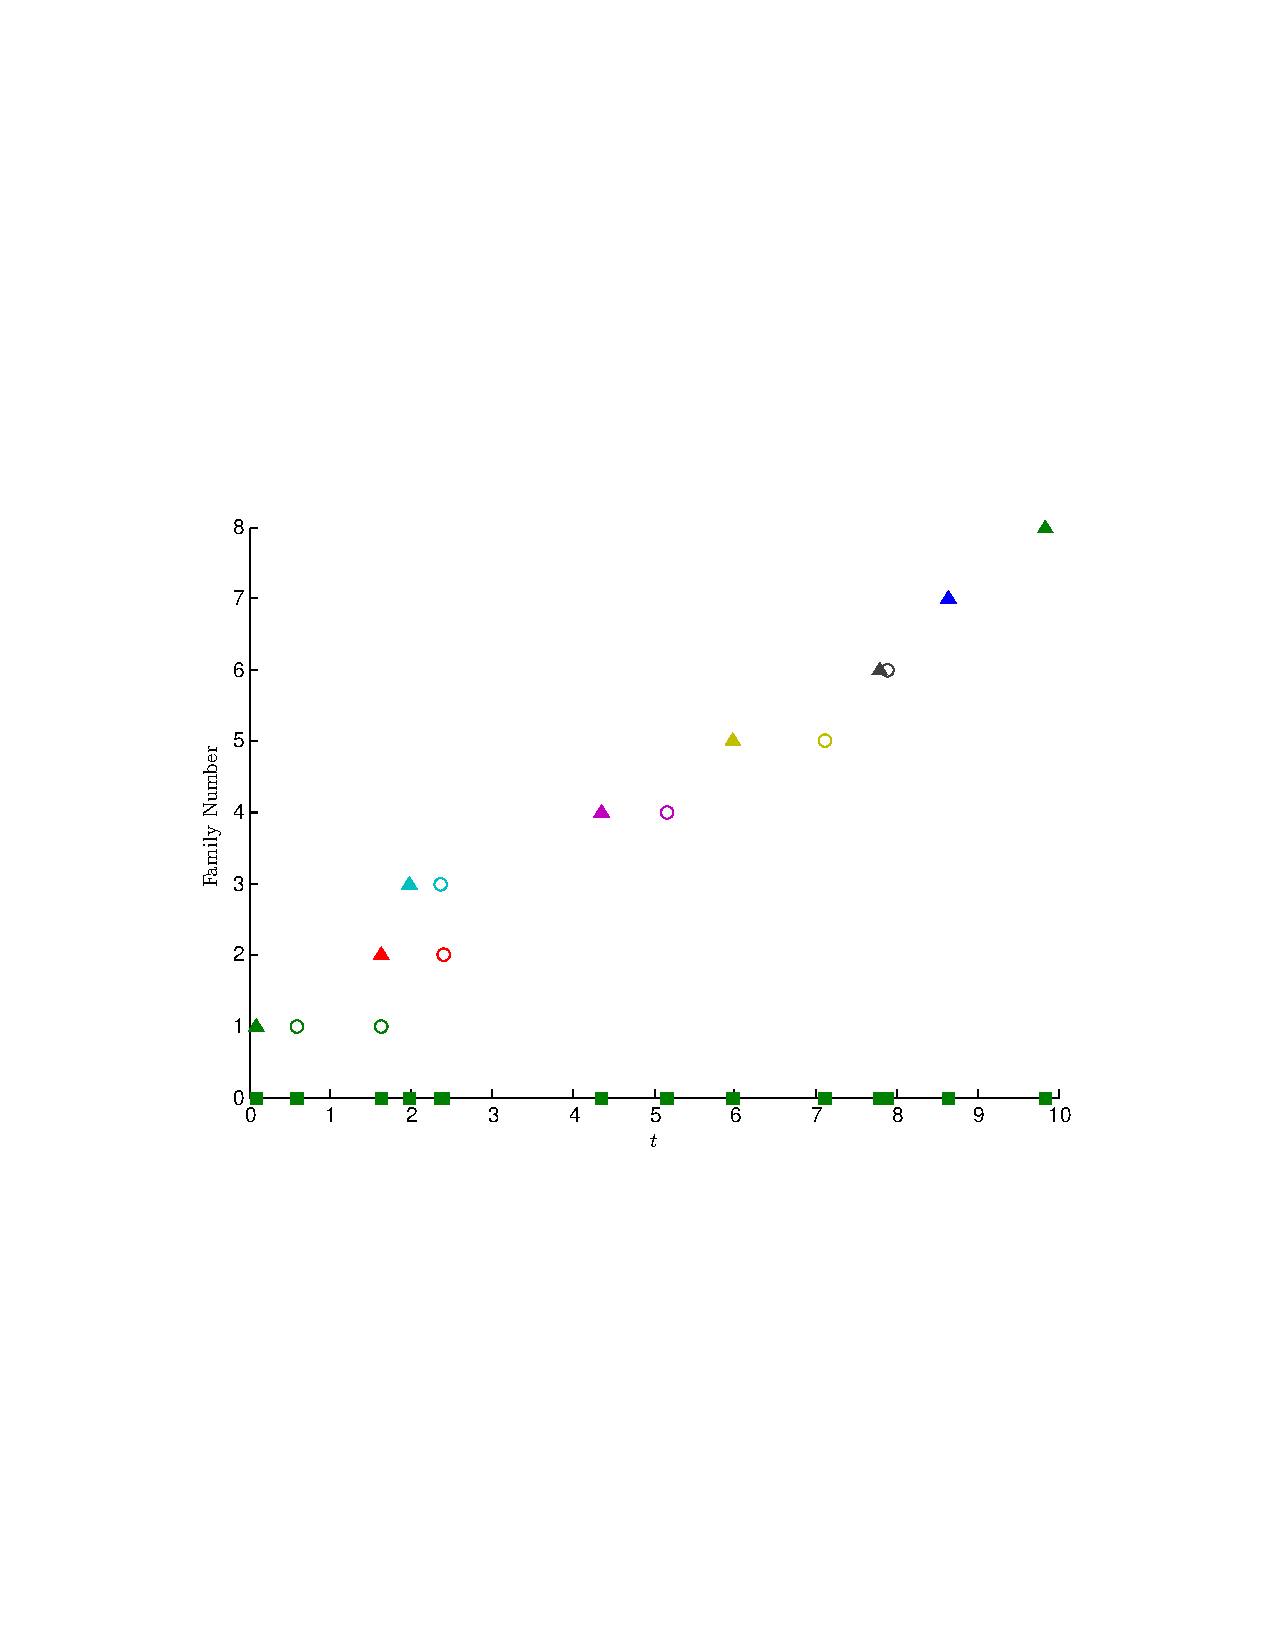
\includegraphics[trim = 0.8cm 8.5cm 0.8cm 8cm,clip,width=1.00\textwidth ]{Hawkess_ClusterFamily.pdf}
	\caption{The points generated by the immigrant–birth representation.}
	\label{Example_ClusterFamily}
\end{figure}
Figure \ref{Example_ClusterFamily} shows the
points generated by the immigrant–birth representation; it can be seen as a sequence
of vertically stacked “family trees”. The immigrant points are plotted as triangles, following circles of the same height and color are its offspring.
\begin{figure}[H]
	\centering
	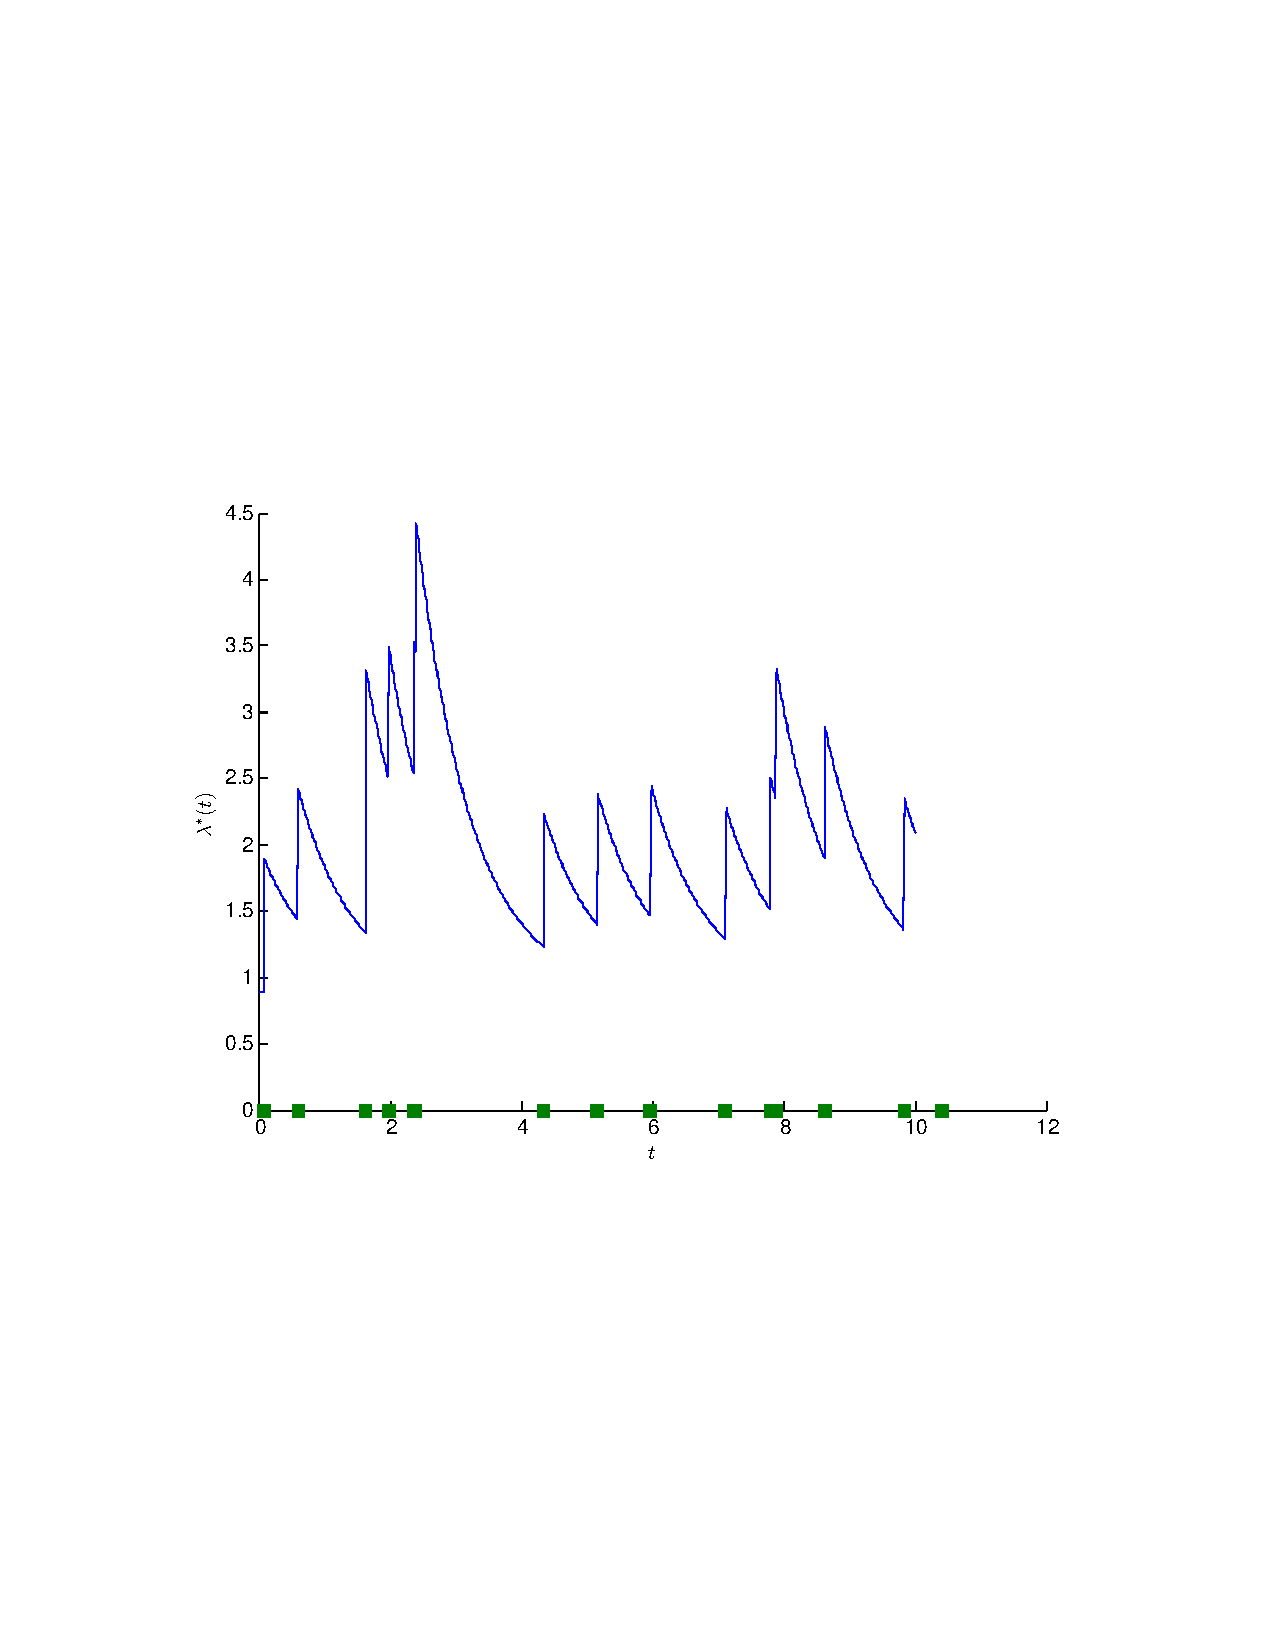
\includegraphics[trim = 0.8cm 8.5cm 0.8cm 8cm,clip,width=1.00\textwidth ]{Hawkess_ClusterIntensity.pdf}
	\caption{The intensity function.}
	\label{Example_ClusterIntensity}
\end{figure}

Figure \ref{Example_ClusterIntensity} shows the intensity function with $(\lambda, \alpha, \beta) = (0.89, 1, 1.2)$. The resulting Hawkes process arrivals are drawn as squares on the axis.